\section*{Appendice}
\addcontentsline{toc}{section}{Appendice}

\begin{figure}[H]
    \centering
    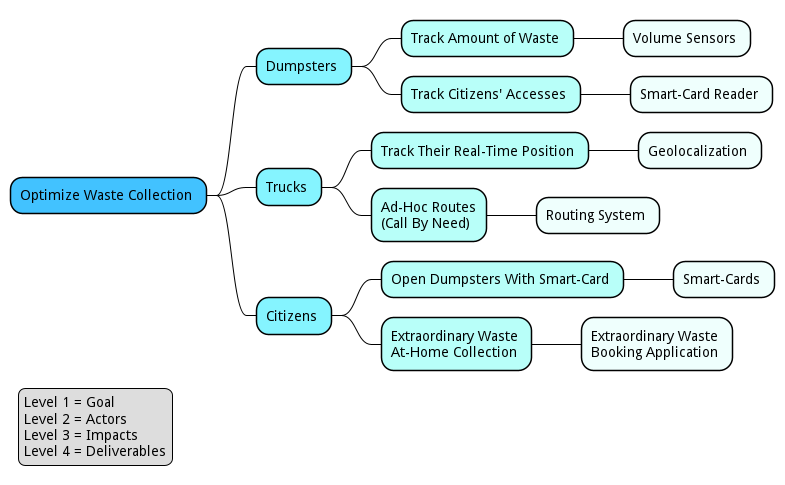
\includegraphics[width=\textwidth]{uml/impact-mapping.pm}
    \caption{\textit{Impact map} che, a partire dal \textit{goal}, mostra quali sono le soluzioni con maggiore impatto sugli attori del sistema.}
    \label{fig:impact-mapping}
\end{figure}


\begin{figure}[H]
    \centering
    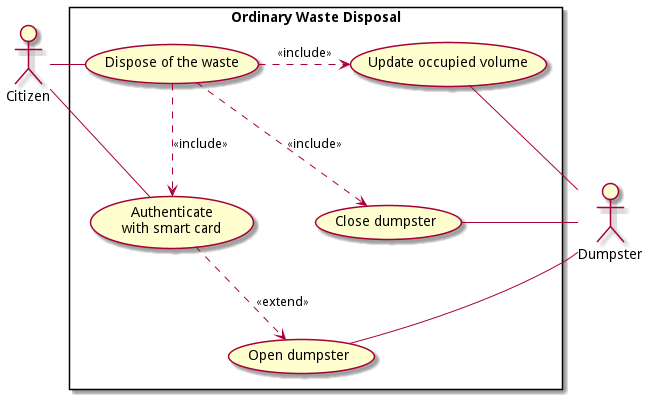
\includegraphics[width=\textwidth]{uml/ordinary-disposal-use-cases.pm}
    \caption{Diagramma dei casi d'uso dello scenario del conferimento di rifiuti ordinari.}
    \label{fig:ordinary-disposal-use-cases}
\end{figure}


\begin{figure}[H]
    \centering
    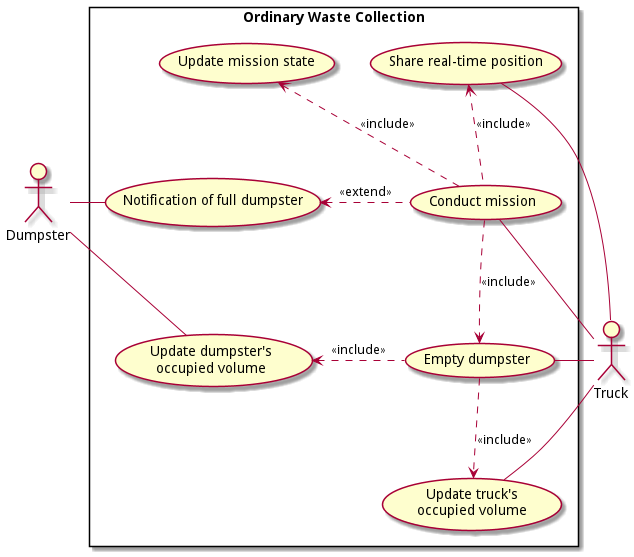
\includegraphics[width=\textwidth]{uml/ordinary-collection-use-cases.pm}
    \caption{Diagramma dei casi d'uso dello scenario della raccolta di rifiuti ordinari.}
    \label{fig:ordinary-collection-use-cases}
\end{figure}


\begin{figure}[H]
    \centering
    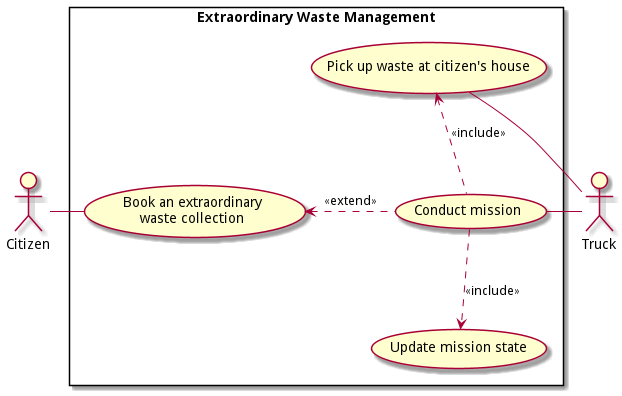
\includegraphics[width=\textwidth]{uml/extraordinary-management-use-cases.pm}
    \caption{Diagramma dei casi d'uso dello scenario della gestione di rifiuti straordinari.}
    \label{fig:extraordinary-management-use-cases}
\end{figure}


\begin{figure}[H]
    \centering
    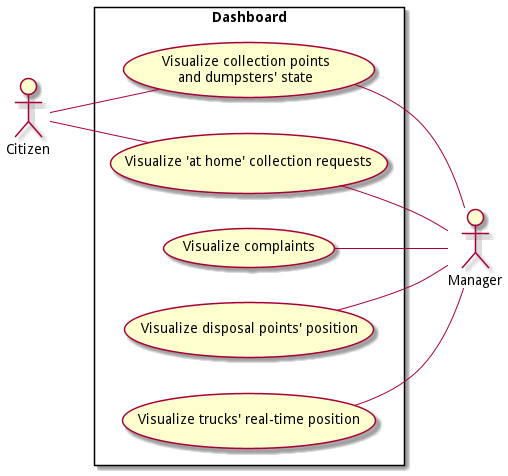
\includegraphics[width=\textwidth]{uml/dashboard-use-cases.pm}
    \caption{Diagramma dei casi d'uso dello scenario dell'utilizzo della dashboard.}
    \label{fig:dashboard-use-cases}
\end{figure}


\begin{figure}[H]
    \centering
    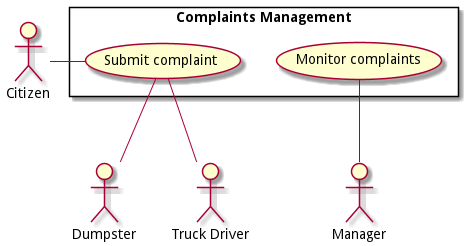
\includegraphics[width=\textwidth]{uml/complaints-use-cases.pm}
    \caption{Diagramma dei casi d'uso dello scenario della gestione dei reclami.}
    \label{fig:complaints-use-cases}
\end{figure}

